\section{Opsætning}

\begin{frame}{Eksperimentel opsætning}
	\begin{columns}
		\column{0.4\textwidth}
		\begin{figure}
			\includegraphics[width=\columnwidth]{../figures/opstilling_better.pdf}
		\end{figure}
		
		\column{0.6\textwidth}
		\small
		\begin{table}
			\begin{tabular}{ll|ll}
				Detektor & Tykkelse {[}$\mu$m{]}  & PAD & Tykkelse{[}$\mu$m{]} \\ \hline
				Det1     & 67                     & n/a & n/a                   \\
				Det2     & 1002                   & P2  & 1036                  \\
				Det3     & 65                     & P3  & 1497                  \\
				Det4     & 60                     & P4  & 1490                  \\
				DetU     & 60                     & PU  & 1498                  \\
				DetD     & 1043                   & PD  & 1038                 
			\end{tabular}
		\end{table}		
	\end{columns}


\end{frame}

\begin{frame}{Detektorer}
	Her er en detektor, den er glad 
\end{frame}